% ============================================================
%  SCHOLA DOMESTICA — Magister Mathematica
%  Level 1 | Week 9 | Day 3
%  Topic: Addition Facts — Sums to 6, Mixed +0–+3; Part-Part-Whole
% ============================================================
\documentclass[12pt, letterpaper]{article}

\usepackage[top=1in, bottom=1in, left=1in, right=1in]{geometry}
\usepackage[T1]{fontenc}
\usepackage[utf8]{inputenc}
\usepackage{lmodern}
\usepackage{microtype}
\usepackage{amsmath}
\usepackage{xcolor}
\usepackage{tikz}
\usepackage{array}
\usepackage{enumitem}
\usepackage{multicol}
\usepackage{mdframed}
\usepackage{fancyhdr}

\definecolor{scholared}{RGB}{160,30,30}
\definecolor{scholagold}{RGB}{180,140,40}
\definecolor{scholacream}{RGB}{253,248,235}
\definecolor{scholagreen}{RGB}{50,110,60}
\definecolor{scholablue}{RGB}{40,80,140}

\pagestyle{fancy}
\fancyhf{}
\renewcommand{\headrulewidth}{0.6pt}
\fancyhead[L]{\small\textcolor{scholared}{\textbf{Schola Domestica — Magister Mathematica}}}
\fancyhead[R]{\small\textcolor{scholared}{Level 1 · Week 9 · Day 3}}
\fancyfoot[C]{\small\textcolor{gray}{— \thepage\ —}}

\newcommand{\answerline}{\underline{\hspace{2.5cm}}}
\newcommand{\biganswerline}{\underline{\hspace{4cm}}}
\newcommand{\numbox}{\tikz{\draw[scholablue,thick](0,0)rectangle(1.2cm,0.85cm);}}

\newmdenv[
  backgroundcolor=scholacream,
  linecolor=scholared,
  linewidth=1.5pt,
  roundcorner=6pt,
  innertopmargin=8pt,
  innerbottommargin=8pt,
  innerleftmargin=10pt,
  innerrightmargin=10pt
]{lessonbox}

\newmdenv[
  backgroundcolor={rgb,255:red,235;green,245;blue,235},
  linecolor=scholagreen,
  linewidth=1.2pt,
  roundcorner=4pt,
  innertopmargin=6pt,
  innerbottommargin=6pt,
  innerleftmargin=8pt,
  innerrightmargin=8pt
]{enrichbox}

\begin{document}

\begin{center}
  {\LARGE\textbf{\textcolor{scholared}{Sums to Six:}}}\\[4pt]
  {\Large\textcolor{scholagold}{\textit{Parts Make a Whole}}}\\[6pt]
  {\small Name: \biganswerline \hspace{1cm} Date: \answerline}
\end{center}

\vspace{4pt}
\noindent\textcolor{scholared}{\rule{\linewidth}{1pt}}
\vspace{4pt}

% IMAGE PROMPT (Miyazaki watercolour style):
% A gentle forest spirit pours small colourful pebbles from two clay pots into a single larger bowl.
% Soft morning light, mossy greens and terracotta tones, white paper background, no text.

\begin{lessonbox}
\textbf{Part + Part = Whole}\\[4pt]
Every addition sentence has two \textbf{parts} that join to make the \textbf{whole}.

\medskip
\noindent
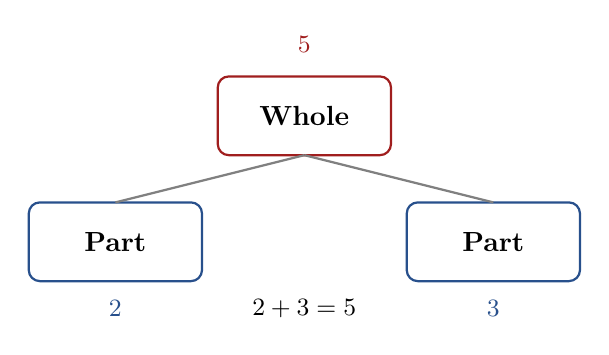
\begin{tikzpicture}
  % Whole box at top
  \draw[scholared, thick, rounded corners=4pt] (3.0, 1.6) rectangle (5.2, 2.6);
  \node at (4.1, 2.1) {\textbf{Whole}};
  % Part boxes
  \draw[scholablue, thick, rounded corners=4pt] (0.6, 0) rectangle (2.8, 1.0);
  \node at (1.7, 0.5) {\textbf{Part}};
  \draw[scholablue, thick, rounded corners=4pt] (5.4, 0) rectangle (7.6, 1.0);
  \node at (6.5, 0.5) {\textbf{Part}};
  % Lines
  \draw[thick, gray] (1.7, 1.0) -- (4.1, 1.6);
  \draw[thick, gray] (6.5, 1.0) -- (4.1, 1.6);
  % Example labels
  \node[scholablue] at (1.7, -0.35) {\small $2$};
  \node[scholablue] at (6.5, -0.35) {\small $3$};
  \node[scholared] at (4.1, 3.0) {\small $5$};
  \node at (4.1, -0.35) {\small $2 + 3 = 5$};
\end{tikzpicture}
\end{lessonbox}

\bigskip

% ===== PART I: FILL IN THE WHOLE =====
\noindent\textcolor{scholared}{\large\textbf{Part I — Find the Whole}} \hfill \textit{(Problems 1–6)}

\medskip
\noindent\textit{The two parts are given. Write the whole (the sum).}

\bigskip

% Part-part-whole diagrams, 2 per row
\noindent
\begin{tabular}{@{}p{7.0cm} p{7.0cm}@{}}

% 1: 2+1=3
\textbf{1.}\quad
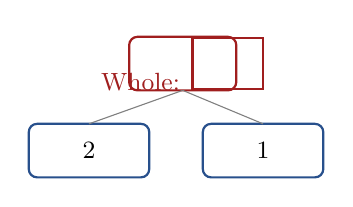
\begin{tikzpicture}[scale=0.85]
  \draw[scholared,thick,rounded corners=3pt](1.5,1.3)rectangle(3.1,2.1);
  \node[scholared] at (2.3,1.7) {\small Whole: \tikz{\draw[scholared,thick](0,0)rectangle(0.9cm,0.65cm);}};
  \draw[scholablue,thick,rounded corners=3pt](0,0)rectangle(1.8,0.8);
  \node at (0.9,0.4) {\small 2};
  \draw[scholablue,thick,rounded corners=3pt](2.6,0)rectangle(4.4,0.8);
  \node at (3.5,0.4) {\small 1};
  \draw[gray](0.9,0.8)--(2.3,1.3); \draw[gray](3.5,0.8)--(2.3,1.3);
\end{tikzpicture}
&
% 2: 3+2=5
\textbf{2.}\quad
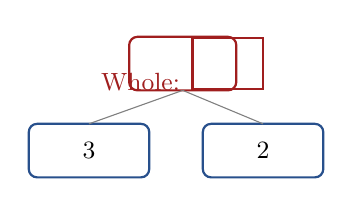
\begin{tikzpicture}[scale=0.85]
  \draw[scholared,thick,rounded corners=3pt](1.5,1.3)rectangle(3.1,2.1);
  \node[scholared] at (2.3,1.7) {\small Whole: \tikz{\draw[scholared,thick](0,0)rectangle(0.9cm,0.65cm);}};
  \draw[scholablue,thick,rounded corners=3pt](0,0)rectangle(1.8,0.8);
  \node at (0.9,0.4) {\small 3};
  \draw[scholablue,thick,rounded corners=3pt](2.6,0)rectangle(4.4,0.8);
  \node at (3.5,0.4) {\small 2};
  \draw[gray](0.9,0.8)--(2.3,1.3); \draw[gray](3.5,0.8)--(2.3,1.3);
\end{tikzpicture} \\[26pt]

% 3: 1+3=4
\textbf{3.}\quad
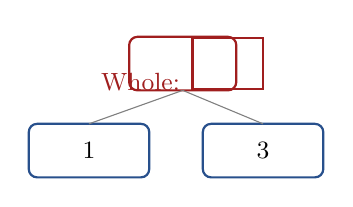
\begin{tikzpicture}[scale=0.85]
  \draw[scholared,thick,rounded corners=3pt](1.5,1.3)rectangle(3.1,2.1);
  \node[scholared] at (2.3,1.7) {\small Whole: \tikz{\draw[scholared,thick](0,0)rectangle(0.9cm,0.65cm);}};
  \draw[scholablue,thick,rounded corners=3pt](0,0)rectangle(1.8,0.8);
  \node at (0.9,0.4) {\small 1};
  \draw[scholablue,thick,rounded corners=3pt](2.6,0)rectangle(4.4,0.8);
  \node at (3.5,0.4) {\small 3};
  \draw[gray](0.9,0.8)--(2.3,1.3); \draw[gray](3.5,0.8)--(2.3,1.3);
\end{tikzpicture}
&
% 4: 0+3=3
\textbf{4.}\quad
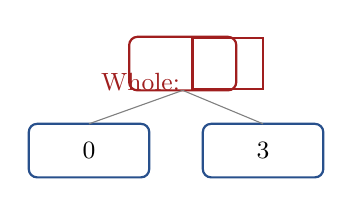
\begin{tikzpicture}[scale=0.85]
  \draw[scholared,thick,rounded corners=3pt](1.5,1.3)rectangle(3.1,2.1);
  \node[scholared] at (2.3,1.7) {\small Whole: \tikz{\draw[scholared,thick](0,0)rectangle(0.9cm,0.65cm);}};
  \draw[scholablue,thick,rounded corners=3pt](0,0)rectangle(1.8,0.8);
  \node at (0.9,0.4) {\small 0};
  \draw[scholablue,thick,rounded corners=3pt](2.6,0)rectangle(4.4,0.8);
  \node at (3.5,0.4) {\small 3};
  \draw[gray](0.9,0.8)--(2.3,1.3); \draw[gray](3.5,0.8)--(2.3,1.3);
\end{tikzpicture} \\[26pt]

% 5: 2+3=5
\textbf{5.}\quad $2 + 3 =$ \numbox
&
% 6: 4+2=6
\textbf{6.}\quad $4 + 2 =$ \numbox

\end{tabular}

\bigskip

% ===== PART II: MIXED FACTS =====
\noindent\textcolor{scholared}{\large\textbf{Part II — Mixed Facts: $+0$, $+1$, $+2$, $+3$}} \hfill \textit{(Problems 7–14)}

\medskip
\noindent\textit{Solve each addition fact. All sums are 6 or less.}

\bigskip

\noindent
\begin{tabular}{@{}p{3.3cm} p{3.3cm} p{3.3cm} p{3.3cm}@{}}
\textbf{7.}\; $5 + 1 =$ \numbox &
\textbf{8.}\; $2 + 2 =$ \numbox &
\textbf{9.}\; $3 + 0 =$ \numbox &
\textbf{10.}\; $0 + 2 =$ \numbox \\[14pt]
\textbf{11.}\; $1 + 3 =$ \numbox &
\textbf{12.}\; $3 + 3 =$ \numbox &
\textbf{13.}\; $4 + 1 =$ \numbox &
\textbf{14.}\; $6 + 0 =$ \numbox
\end{tabular}

\bigskip

% ===== PART III: WORD PROBLEMS =====
\noindent\textcolor{scholared}{\large\textbf{Part III — Story Problems}} \hfill \textit{(Problems 15–16)}

\medskip

\noindent\textbf{15.} Peter has \textbf{3} carrots. His sister gives him \textbf{2} more. How many carrots does he have?

\medskip
\noindent\hspace{2em} Write the addition sentence: $\numbox + \numbox = \numbox$

\bigskip

\noindent\textbf{16.} There are \textbf{4} butterflies on a flower. One more lands. How many butterflies?

\medskip
\noindent\hspace{2em} $\numbox + \numbox = \numbox$ butterflies

\bigskip

\begin{enrichbox}
\textbf{\textcolor{scholagreen}{Oral Drill — Parts to 6}}\\[3pt]
Teacher reads the problem; child says the answer aloud.\\[4pt]
\noindent
$3{+}1$ \quad $2{+}2$ \quad $0{+}3$ \quad $1{+}2$ \quad $4{+}0$ \quad $2{+}3$ \quad $3{+}3$ \quad $5{+}1$\\[2pt]
\textit{Repeat the row until your child answers without hesitation.}
\end{enrichbox}

\vspace{0.3cm}
\noindent\textcolor{gray}{\small\textit{Ray's Primary Arithmetic — joining parts to make a whole.}}

\end{document}
